\documentclass{article}

% Language setting
% Replace `english' with e.g. `spanish' to change the document language
\usepackage[english]{babel}

% Set page size and margins
% Replace `letterpaper' with `a4paper' for UK/EU standard size \usepackage[letterpaper,top=2cm,bottom=2cm,left=3cm,right=3cm,marginparwidth=1.75cm]{geometry}
% Useful packages
\usepackage{amsmath}
\usepackage{graphicx}
\usepackage{multirow}
\usepackage{booktabs}
\usepackage[colorlinks=true, allcolors=blue]{hyperref}

\title{Video Query Processing with Text}
\author{Sinclair Hudson}

\begin{document}
\maketitle

\begin{abstract}
      This work explores different ways to leverage large language models (LLMs) to convert video into textual descriptions, and then further answer queries about the video using the textual descriptions.
\end{abstract}

\section{Introduction}

We propose a video understanding pipeline using LLMs that can be used to...
% TODO hmmm
Simultaneously, the performance of language models has surged in recent years, largely thanks to the predictable scaling of transformer-based models.
This work proposes a general pipeline for accomplishing video understanding tasks using multimodal LLMs, by converting visual information into text.

\section{Related Work}

CLIP4CLIP is a method that aims to extend the ideas of CLIP \cite{clip} to the video domain \cite{clip4clip}.
It generally follows a bi-encoder structure, in which the video and text are encoded using separate transformers \cite{transformer}. Then, both representations are fed into a similarity calculator module.
The system is trained end-to-end with contrastive loss, as in CLIP \cite{clip}.

XCLIP \cite{xclip}

InternVideo is a recent attempt at a "foundation model" for video, being able to complete numerous downstream tasks.
The authors train InternVideo with a combination of multimodal constrastive learning (as in CLIP \cite{clip}), as well as masked video reconstruction, inspired by VideoMAE \cite{videomae}.


\subsubsection{Multi-Modal Large Language Models}

\subsection{Video Retrieval}

\subsection{Video-Text datasets}
MSR-VTT (Microsoft Research Video to Text) is a popular video understanding dataset \cite{msr-vtt}.
This dataset can be used for multiple tasks, including Video Question Answering, Video Retrieval, and Video Captioning.
The dataset contains 10,000 videos, largely sourced from the internet (TODO verify).
For the video retrieval task, 1000 queries are used for testing, each specifying exactly one video as the correct answer \cite{jsfusion}.
The videos in the video retrieval task are 12 seconds long on average, see \ref{fig:length_histogram} for a histogram of video lengths.

\begin{figure}
      \centering
      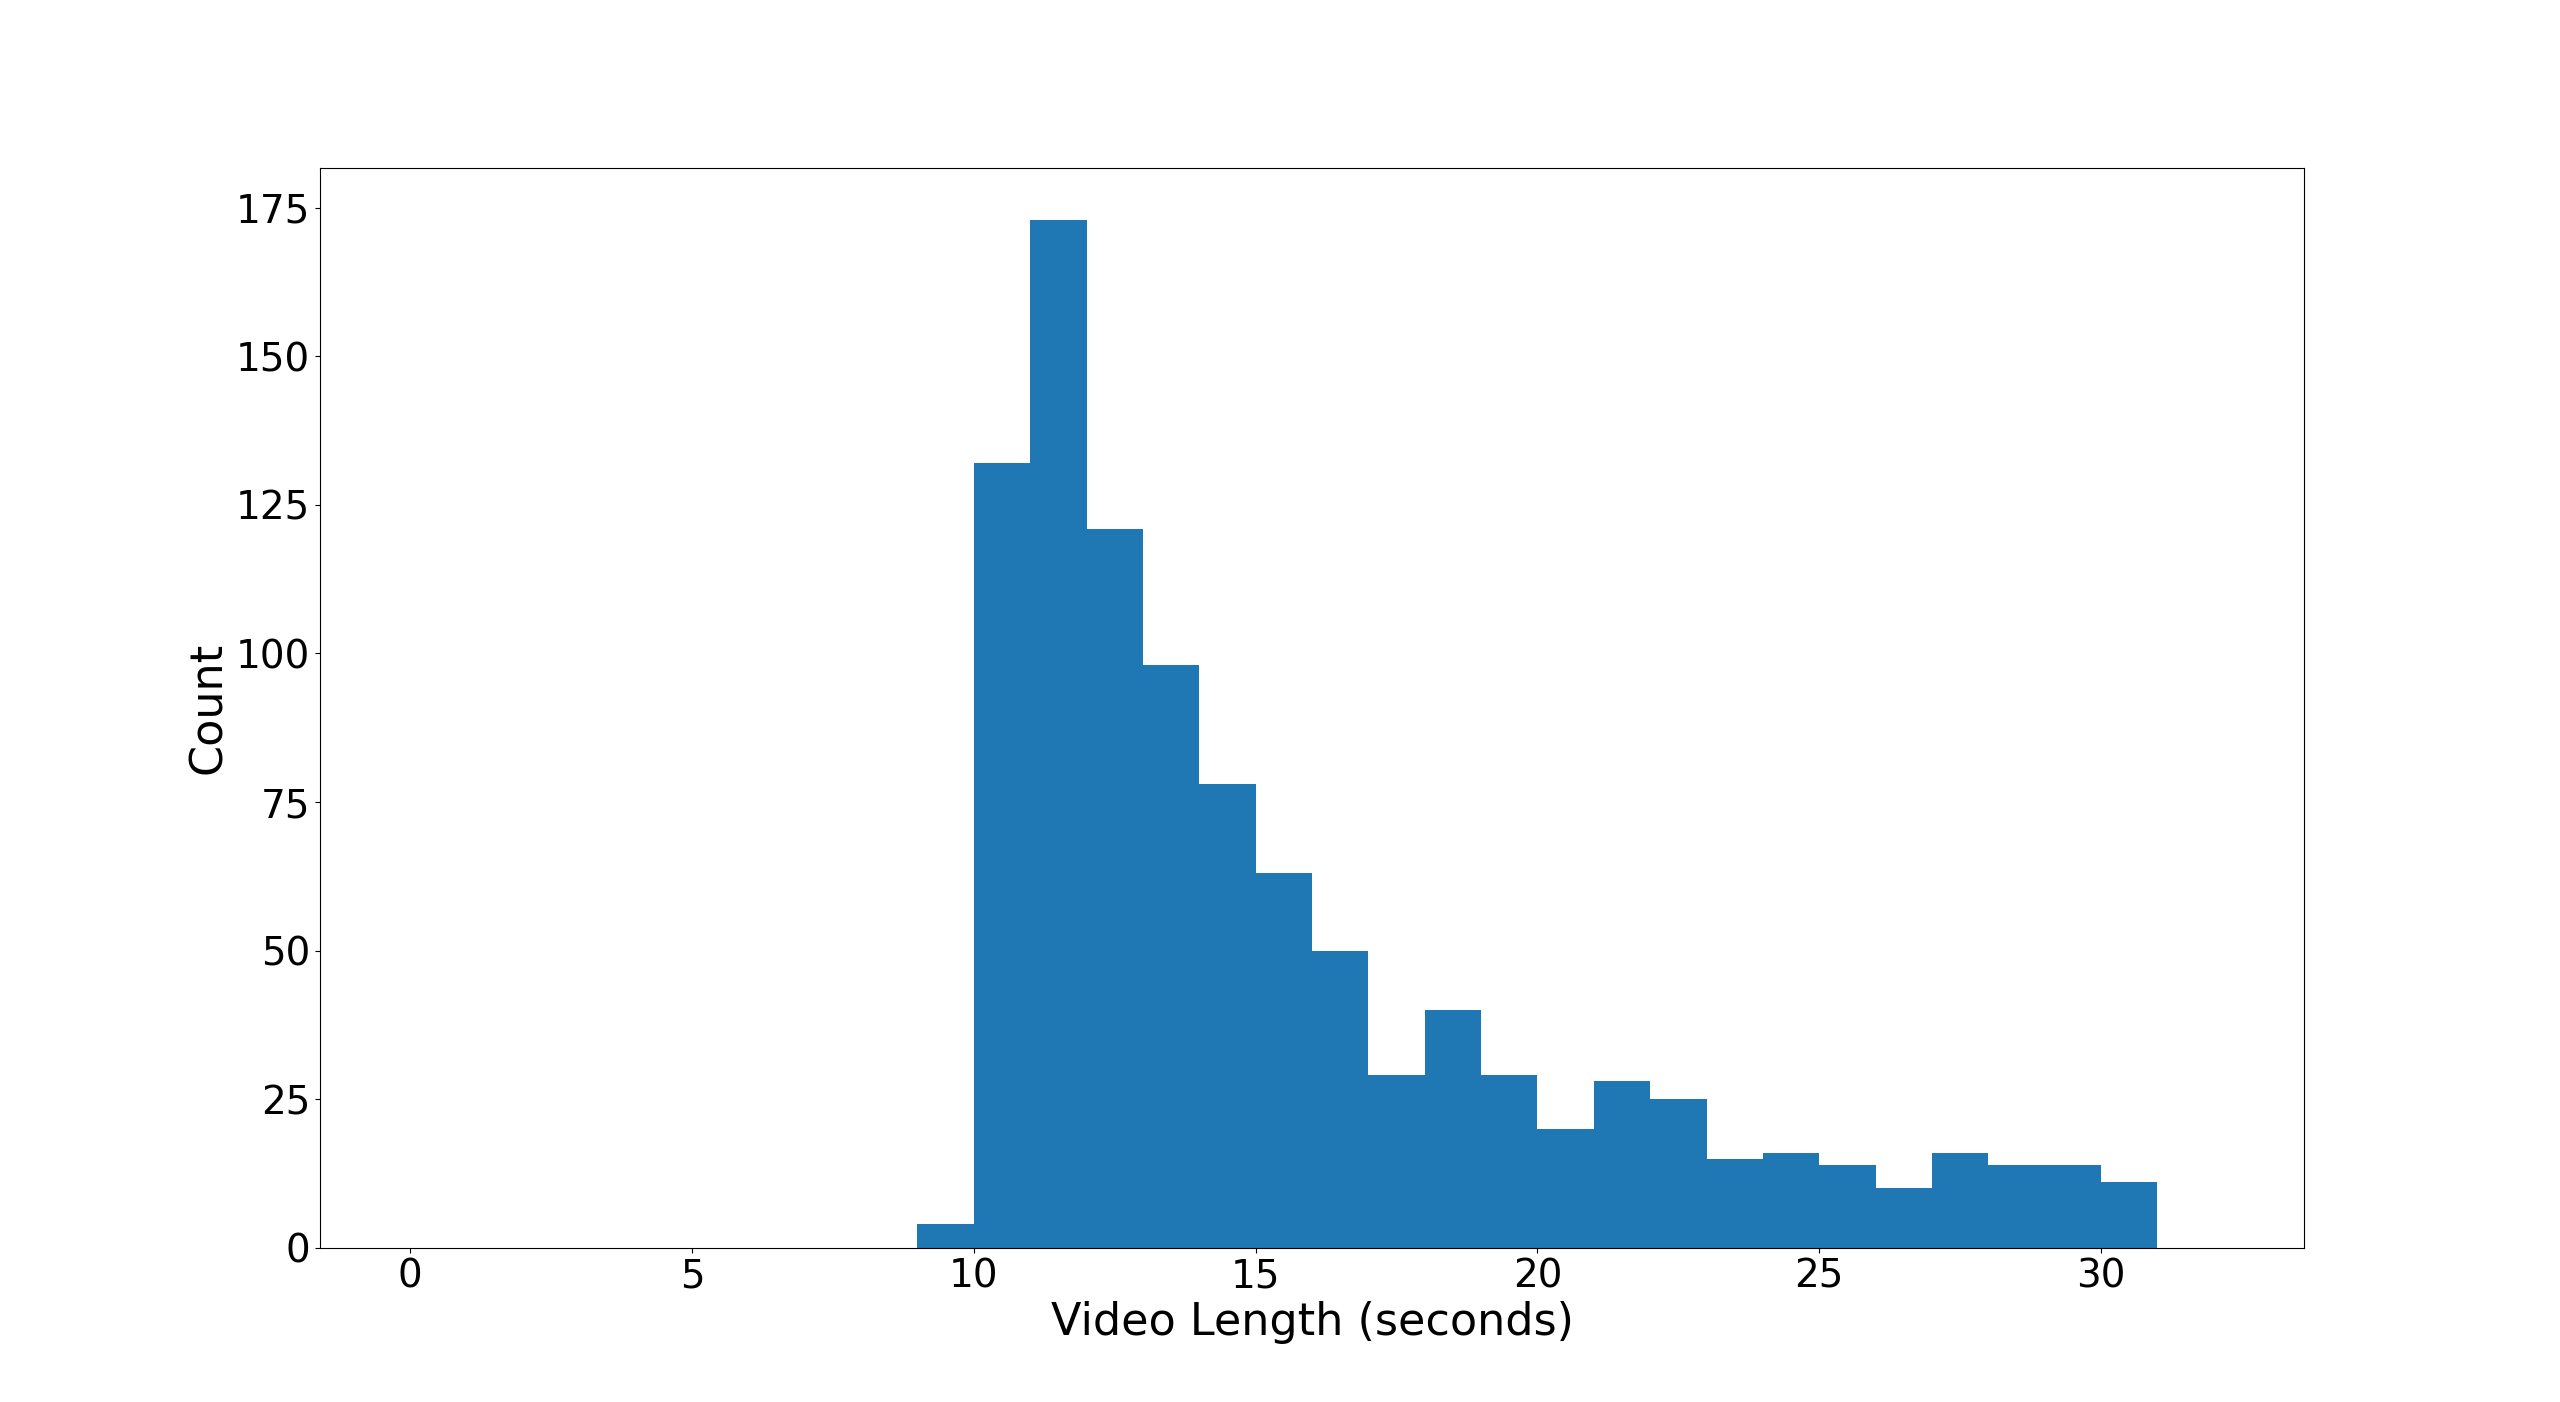
\includegraphics[width=0.8\textwidth]{figures/msr-vtt-length-histogram.png}
      \caption{Length of videos in the MSR-VTT retrieval data split.}
      \label{fig:length_histogram}
\end{figure}

\section{Pipeline}

%TODO figure here
%\caption{The high level pipeline to use LLMs to understand video.}

For the purposes of this work, a "clip" is a small segment of a video that is a few seconds long, 
and is highly cohesive in what it depicts. For example, in a movie, a clip might be a single shot.
At a high level, the pipeline for video understanding using LLMs is as follows:
\begin{enumerate}
      \item Partition the video into individual clips (optional)
      \item From each clip, select a small subset of frames to represent the clip
      \item Using the selected frames, generate a textual description of the clip using an LLM.
      \item Using the textual description, answer queries about the video, or retrieve clips.
\end{enumerate}

For brevity, these steps will be referred to as "Clip partitioning", "Frame selection", "Clip description", and "Clip Retrieval" respectively.
The two most applicable tasks for this pipeline are video retrieval and video summarization.
In video retrieval, given a query, the goal is to retrieve the video in a video dataset that best matches the query.
In visual video summarization, the goal is to edit a video down to a shorter length, containing only clips relevant to a given query.



\section{Clip Partitioning}

Videos can contain a lot of different clips, which may or may not be related.
The input for clip partitioning is the whole video, and the output is a list of breaks (frame numbers) between clips.
The difficult aspect of clip partitioning is to efficiently find the boundaries between clips.
A two-hour video at 24 frames per second contains 172,800 frames, and so processing each one is computationally expensive.
\subsection{Uniform partitioning}
The simplest approach to clip partitioning is to simply partition the video into equal-sized clips, without regard for the content of the video.
This approach is simple, but the resulting clips are not necessarily cohesive, since clips could contain multiple scenes and shots.
\subsection{Coarse-to-fine clip partitioning}
Starts by computing the L1 distance between frames 1 second apart.
If the the distance is above a certain threshold, then a clip break is likely in this second.
Thus, the 1-second segment is evaluated frame by frame, and if the distance between two frames is above a threshold, then a clip break is identified.

\begin{figure}
      \centering
      \includegraphics[width=0.8\textwidth]{figures/TODO.png}
      \caption{Frames one before and one after a clip break, determined by the coarse-to-fine clip partitioning strategy. The movie being partitioned is TODO}
      \label{fig:optical_flow}
\end{figure}


\section{Frame Selection}

Even within a single clip, there are a lot of frames, most of which are very similar to their neighbours.
To make the pipeline efficient, it's critical to select the subset of the most semantically relevant frames.
LLMs can only effectively interpret one image at a time (todo verify).
The input to frame selection is a clip (small length of video) and the output is a list of frames selected for further processing.

Earlier works simply sample randomly \cite{TODO} or sample uniformly, at a course framerate such as 1 frame per second \cite{clip4clip}.

This work explores 3 different frame selection strategies:
greedy L1 selection, stratified sampling, and TODO.

\subsection{Stratified Sampling}
To get a potentially more diverse set of frames, the first, last and middle frames are selected.
We call this sampling method \verb|3-strat|. We also explore \verb|5-strat|, which selects the first, last, and 3 evenly spaced frames in between.

\subsection{Stratified Triplet Sampling}
It's possible that the stratified sampling method above is too coarse, and that a single frames at multiple points in the clip is not enough to capture the clip's content.
For this reason, this work also explores stratified triplet sampling, where at each of the 3 points in the clip, 3 frames are selected across 1 second.
The motivation for this method is that the 3 frames in a single second will show what is changing in the scene.
each triplet is fed in as a single input into the LLM, which can take multiple images as input.
As a result, there is only one textual description per triplet in this sampling method.

\subsection{Greedy L1 Selection}
Greedy L1 selection initially selects the first frame of a clip. Then, it selects an additional clip if the L1 distance between the new frame and the previously selected frame is greater than some threshold (for example).
The L1 distance is normalized by the number of pixels in the image, so that the threshold is independent of the video resolution.
In the MSR-VTT dataset, most videos are quite short (TODO graph for this), and often only contain a single shot.
As such, when using Greedy L1 selection, a substantial number of videos only have the first frame selected (with L1 threshold 180).
The idea for selction based on L1 is to skip frames that are visually similar to the previously selected frame.
The selection strategy is greedy; the first frame is always selected, and then frames are considered in order, only selected if the frame differs from the previously selected frame by a certain L1 distance.
More formally

% TODO maybe just write an algorithm block for this? It's not difficult
\begin{equation}
      c < \frac{|I_{p} - I_{c}|}{W \times H \times C}
\end{equation}
where $c$ is a pre-defined threshold, $I_{p}$ is the previously selected frame, $I_{c}$ is the current frame, and $W$, $H$, $C$ are the width, height, and channels of the frames, respectively.

\begin{figure}
      \centering
      \includegraphics[width=0.8\textwidth]{figures/L1_frame_selection.png}
      \caption{Number of frames selected per video in the MSR-VTT dataset retrieval split, for different thresholds.}
      \label{fig:optical_flow}
\end{figure}

L1 was chosen over L2 because L2 is very sensitive to large changes in a few pixels; L1 gives a better sense of the overall change in the image.

\section{Prompting Strategies}

The LLM used in testing this pipeline is LLava \cite{llava}.
LLaVA is selected because it is free and open source, and can be run on a single consumer GPU, making it amenable to experimentation.

Beam search, multiple prompts with a temperature.
Two prompts are tried in this work, one of which is is dubbed "concise" (C), while the other is "verbose" (V).
The concise prompt is ""
The verbose prompt is "Please describe the objects in this image. Be as descriptive as possible."
For getting a textual description of a single image, the prompt used is "Please describe the objects in this image. Be as descriptive as possible.".
LLM performance can be sensitive to prompts.

The input to the LLM is a prompt and (potentially) multiple frames, and the output is a text caption.
In all cases, we limit the length of the caption to 512 words, to bound the amount of computation required per frame.

\section{Retrieval}

The last aspect of 

Because LLMs have described the content of the videos, the retrieval task is reduced to that of text retrieval, which is well-studied.
In this work, we explore two retrieval strategies: BM25 and Dense Passage Retriever (DPR).
BM25 is a highly performant sparse retriever, relying on term frequencies TODO.
DPR is a dense retriever, which uses a neural network to embed the query and the documents into a vector space, and then uses cosine similarity to retrieve the most similar documents to the query.

\section{Results}

\begin{table}[htbp]
  \centering
  \begin{tabular}{lcccc}
    \toprule
    \textbf{Benchmark} & \multicolumn{3}{c}{\textbf{MSR-VTT}} \\
    \cmidrule(lr){2-4}
    & \textbf{R@1} & \textbf{B} & \textbf{C} \\
    \midrule
    \multirow{2}{*}{CLIP4Clip} & 0.85 & 0.88 & 0.90 \\
    & (0.02) & (0.01) & (0.03) \\
    \midrule
    \multirow{2}{*}{XCLIP} & 0.78 & 0.82 & 0.85 \\
    & (0.03) & (0.02) & (0.01) \\
    \midrule
    \multirow{2}{*}{InternVideo} & 0.92 & 0.89 & 0.91 \\
    & (0.01) & (0.02) & (0.01) \\
    \bottomrule
  \end{tabular}
  \label{tab:model_comparison}
  \caption{Performance Comparison of Models on Different Benchmarks}
\end{table}

\subsection{Qualitative Results on video summarization}
For video summarization, the task is to select a subset of clips from a video relevant to the query.
Sports games are desireable to summarize because they are long, with a few well-defined interesting events (goals, fouls, etc.).
To test this method, we will full sports games from YouTube.
In this full soccer game, 7 goals are scored, 4 by France and 3 by Argentina.

\begin{table}[htbp]
  \centering
  \begin{tabular}{lcccc}
    \toprule
    \textbf{Query} & \multicolumn{3}{c}{\textbf{MSR-VTT}} \\
    \cmidrule(lr){2-4}
    & \textbf{Event Recall} & \textbf{Summary video length} & \textbf{C} \\
    \midrule
    \multirow{2}{*}{Goals Scored by team France, in dark blue jerseys.} & 0.85 & 0.88 & 0.90 \\
    & (0.02) & (0.01) & (0.03) \\
    \midrule
    \multirow{2}{*}{Goals scored by team Argentina, in light blue and white jerseys.} & 0.78 & 0.82 & 0.85 \\
    & (0.03) & (0.02) & (0.01) \\
    \midrule
    \multirow{2}{*}{Goals scored by either team} & 0.92 & 0.89 & 0.91 \\
    & (0.01) & (0.02) & (0.01) \\
    \bottomrule
  \end{tabular}
  \label{tab:video_summarization}
  \caption{Performance Comparison of Models on Different Benchmarks}
\end{table}

\section{Discussion}


\section{Future work}

Expanding methodologies to other datasets is critical to fully examine the generalization capability of these pipelines.
Additionally, this pipeline currently is very slow, requiring many forward passes of a large language model for every frame, and multiple frames for every clip.
Future work could investigate further minimizing the number of frames processed, and prompting techniques to generate very dense captions, with a lot of information content in few tokens.
Finally, while this work focused on the visual features of video, audio is also often attached to video, and thus could be used to further improve the performance of the pipeline.
Related work such as TODO has shown that audio can provide a small boost to performance \cite{TODO}.

\section{Conclusion}

\bibliographystyle{alpha}
\bibliography{biblio}

\end{document}
